\section{A Comparison of Tendencies}

I attempted to distinguish between the linguistic tendencies of King Crimson and Johnny Cash|progressive rock and folk/country artists respectively|using the tools learnt in this module.

\subsection{Gathering and processing of data}
\subsubsection{Retrieval of lyrics}

\paragraph{Download}

The songs were downloaded from \href{https://genius.com/}{genius.com} with the code shown in \cref{lst:get songs}. The api used is documented in \cite{geniusapi}. The structure of the function shown in \cref{lst:get songs} is as follows:
\begin{itemize}
	\item[\texttt{ll:2-8}] Setup api metadata and song storage location.
	\item[\texttt{ll:10-15}] The song list for each artist was set up to be accessed page-by page, with the maximum page size being fifty songs. Here, the first page is retrieved, using the python \texttt{requests} library.
	\item[\texttt{l:16}] The data structure returned by the \texttt{GET} request for an artists songs has a field corresponding to the index of the next page, if one exists. Here, that index is used to test whether or not the last page has been processed.
	\item[\texttt{ll:17-19}] Sim. ll. 13-15.
	\item[\texttt{l:20}] Advance the page count for the next iteration.
	\item[\texttt{ll:22-32}] A loop over those songs returned that match the id of the artist requested and whose lyrics were complete, i.e. not in progress. If the song has not already been downloaded|no file exists that matches its proposed filename|it will be downloaded as shown, using the \texttt{BeautifulSoup} library \cite{beautifulsoup} to retrieve the lyrics from the webpage at the url retrieved from the earlier json object.
\end{itemize}

\paragraph{Presentation as useful data}

I used a pair of classes, \texttt{Song} and \texttt{Artist} (\cref{lst:artist,lst:song}), to perform the filtering and organisation of the lyric data.


The \texttt{Artist} class (\cref{lst:artist}) essentially just creates a list of song objects from filenames that match a certain pattern corresponding to one of its songs.

The \texttt{Song} class (\cref{lst:song}) has more functions, some of which are used later for the analysis of the artists' work.
\begin{itemize}
	\item[\texttt{2-8}] \texttt{\textunderscore \textunderscore init\textunderscore \textunderscore }\\ Constructor of \texttt{Song}. Stores pre-downloaded lyrics as tokenised words. The weakness of this approach is that \texttt{\texttt{nltk.word\textunderscore tokenise}} splits on punctuation, such that words like "can't" and "don't" become \texttt{['can',"'t"]} and \texttt{['don',"'t"]}.
	\item[\texttt{10-14}] \texttt{from\textunderscore file}\\
	Alternate factory method of \texttt{Song} to construct the class from  a given filename, parsing the title and artist from said filename.
	\item[\texttt{16-17}] \texttt{filtered}\\
	Render the raw token list of the song's lyrics into a form more suitable for analysis:
	\begin{itemize}
		\item Filter out punctuation. The analyses performed operate on words; the idiosyncrasies of each artists' punctuation styles are irrelevant. Were analyses to be performed on, for example, how the artist might begin a sentence, this step would be removed.
		\item Filter out words that do not add information but rather facilitate communication between people. These words would not help to spot any meaningful distinction between the artists' styles or help find some theme in their work as they are common to most works.
	\end{itemize}
	\item[\texttt{22-25}] \texttt{filename\textunderscore fmt}\\
	Return a path that will match a file or files corresponding to the author and title given.
\end{itemize}

 Once downloaded, a list of artists was compiled from the downloaded lyrics as shown in \cref{lst:make artists}.
\begin{listing}[h]
\begin{minted}{python}
artists = ["King Crimson","Johnny Cash"]
aa = [Artist(a) for a in artists]
\end{minted}
\caption{Creating a list of artists. For the definition of \texttt{Artist} see \cref{lst:artist}.}
\label{lst:make artists}
\end{listing}
\begin{listing*}%
	\centering%
	\caption{Listing for \texttt{Song}, the class managing retrieval and processing of song lyrics.}%
	\inputminted{python}{src/Song.py}
	\label{lst:song}%
	\hrule
\end{listing*}
\subsection{Analysis}
Once the artists' data had been rendered into a usable format, the analyses could be performed.

Some analyses were performed on the entirety of an artist's recorded body of work. These corpora were generated as shown in \cref{lst:bow gen}.

\begin{listing}[h]
\begin{minted}{python}
artist_bow = [None] * len(aa)
for i,a in enumerate(aa):
	words = []
	for s in a.songs:
		words.extend(s.filtered())
		artist_bow[i] = words
\end{minted}
\caption{Generation of master list of artists' lyrics.}
\label{lst:bow gen}
\end{listing}

\subsubsection{Methods}
While some of the below methods of analyses provided good insight into the distinguishing features of each artist's work, combinations proved to be the most helpful, for example stemming words before applying a frequency distribution to the stemmed words.
\paragraph{Frequency Distribution}

The \texttt{nltk.FreqDist} class constructs a frequency distribution of a list of tokens, i.e. a set of words and their corresponding number of occurrences in the list of tokens. Its plot method was often used in this assignment. Plots of the frequency distribution of words from each artist's work are given in \cref{fig:freq dist JC,fig:freq dist KC}. 

\paragraph{Stemming} is the process of finding a root form or stem for each word in order to reduce or ideally eliminate duplicates from consideration. \Cref{lst:stemming} shows the procedure followed throughout this assignment. Below, where a variable has been suffixed with \texttt{\textunderscore stem}, the words in that list have undergone this process.
\begin{listing}[h]
\begin{minted}{python}
porter = nltk.PorterStemmer()
artist_bow_stem = 
	[[porter.stem(w) for w in bow]
	 for bow in artist_bow]
for stem in artist_bow_stem:
	nltk.FreqDist(stem).plot(15)
	\end{minted}
	\caption{Stemming and its effect on the frequency distribution of the artists' lyrics. \Cref{fig:freq dist JC stem,fig:freq dist KC stem} show the new frequency distributions after stemming.}
	\label{lst:stemming}
\end{listing}

\paragraph{Lexical Diversity}

Lexical diversity, as defined in \cref{lst:lex div}, is the ratio of the number of unique words in a text to the length of said text. It is a measure of the complexity of the text.

I aimed to use it as a means of distinguishing songs from the different artists on the premise that one artist's work would be more lexically diverse than the other. This premise seems to have proved true: although I haven't assessed the degree of the distinction, the lexical diversity of King Crimson's work|when taken over their whole corpus|is 68.53\% greater than that of Johnny Cash's (see \cref{lst:lex div overall}).

A similar relationship exists when lexical diversity is evaluated over each song. Two measures of central tendency, the arithmetic mean and the median, show a significantly greater average lexical diversity for King Crimson's work.

If the lexical diversity of the songs is normally distributed, then due to the lower mean and smaller standard deviation, the work of Johnny Cash is once more less lexically diverse than that of King Crimson; these normal distributions could be used to predict the likelihood of a given song belonging to one or another artist.

\begin{listing}[h]
\begin{minted}{python}
def lexical_diversity(text):
	return len(set(text)) / len(text)
\end{minted}
\caption{Definition of lexical diversity.}
\label{lst:lex div}
\end{listing}

\begin{listing}[h]
	\begin{minted}{python}
for art,bow in zip(artists, artist_bow):
print(f"LEXICAL DIVERSITY OF {art}: {lexical_diversity(bow)}")
	\end{minted}
	\centering
	\begin{tabular}{lc}
		\toprule
		Artist&Lexical Diversity\\
		\cmidrule(r){1-1}\cmidrule(l){2-2}
		King Crimson&0.2819\\
		Johnny Cash&0.0887\\
		\bottomrule
	\end{tabular}
	\caption{Overall lexical diversity of artists.}
	\label{lst:lex div overall}
\end{listing}

\begin{listing}[h]
\begin{minted}{python}
import statistics as stats
for a,llex in zip(aa,lexdiv_stem):
	print(f"==>ARTIST:{a.name}")
	print(f">MEAN {stats.mean(llex)}")
	print(f">SD {stats.stdev(llex)}")
	print(f">MEDIAN{stats.median(llex)}")
\end{minted}
	\centering
\begin{tabular}{lcc}
	\toprule
	Measure&King Crimson&Johnny Cash\\
	\cmidrule(r){1-1}\cmidrule(lr){2-2}\cmidrule(l){3-3}
	$\bar{x}$&0.7250&0.6580\\
	$\sigma_x$&0.2116&0.1428\\
	$median\{x\}$&0.7554&0.6724\\
	$min\{x\}$&0.2400&0.2000\\
	\bottomrule
\end{tabular}
\caption{Statistical lexical diversity over individual songs using the \texttt{statistics} library~(top); output statistics (bottom).}
\label{lst:songs lex div}
\end{listing}

\paragraph{Collocations}

\Cref{lst:colloc find} shows the code used to find collocations in both artists' bodies of work and \cref{lst:colloc find out} shows the collocations found\footnote{This code is adapted from some at \cite{collocations-nltk}. The idea to use collocations comes from Workshop One.}. These proved to be a great means to distinguish the two artists: among the words most correlated in King Crimson's oeuvre being the more violent bigrams and trigrams of \texttt{('greed','poets')} and \texttt{('barbed','wire','politicians')}; the collocations resulting from Johnny Cash's work on the other hand had a more folk, religious and American country music feel with examples like \texttt{('redeemer','beckoning')} and \texttt{('waving','patriotic','nephew')}.

This means of measurement seemed to provide the most distinction between the artists. Given the most correlated bigrams in a new song, I feel I would be able to guess reasonably accurately to which artist it belonged.

\begin{listing}[h]
	\begin{minted}{python}
bigram = nltk.collocations.BigramAssocMeasures()
trigram = nltk.collocations.TrigramAssocMeasures()

bfinders = [BigramCollocationFinder.from_words(bow) for bow in artist_bow]
tfinders = [TrigramCollocationFinder.from_words(bow) for bow in artist_bow]
for finder in bfinders:
	finder.apply_freq_filter(5)
	print(finder.nbest(bigram.pmi, 10))
for finder in tfinders:
	finder.apply_freq_filter(5)
	print(finder.nbest(trigram.pmi, 10))
	\end{minted}
\caption{Finding collocations in both bodies of work. For output, see \cref{lst:colloc find out}.}
\label{lst:colloc find}
\end{listing}

\begin{listing}
	\begin{BVerbatim}
# King Crimson
[('greed', 'poets'), ('innocents', 'raped'), 
('poets', 'starving'), ('pyre', 'innocents'),
('schizophrenic', 'tendencies'), ('barbed', 'wire'),
('paranoia', 'poison'), ('raped', 'napalm'),
('wire', 'politicians'), ('prince', 'rupert')]
#Johnny Cash
[('boa', 'constrictor'), ('chandeliers', 'burgundy'),
('redeemer', 'beckoning'), ('sandy', 'scag'),
('patriotic', 'nephew'), ('honky', 'tonk'),
('rick', 'rubin'), ('orange', 'blossom'),
('wondrous', 'waddy'), ('wooly', 'booger')]
# King Crimson
[('greed', 'poets', 'starving'), 
('pyre', 'innocents', 'raped'),
('barbed', 'wire', 'politicians'), 
('innocents', 'raped', 'napalm'),
('many', 'schizophrenic', 'tendencies'),
('funeral', 'pyre', 'innocents'),
('politicians', 'funeral', 'pyre'),
('poets', 'starving', 'children'),
('scream', 'paranoia', 'poison'),
('wire', 'politicians', 'funeral')]
# Johnny Cash
[('crystal', 'chandeliers', 'burgundy'),
('produced', 'rick', 'rubin'),
('waving', 'patriotic', 'nephew'),
('patriotic', 'nephew', 'uncle'),
('orange', 'blossom', 'special'),
('drunken', 'ira', 'hayes'),
('drifter', 'driftin', 'drifter'),
('slapped', 'shoe', 'polish'),
('ends', 'tie', 'binds'), 
('flag', 'waving', 'patriotic')]
	\end{BVerbatim}
	\caption{Collocations found in bodies of work. Output of \cref{lst:colloc find}.}
	\label{lst:colloc find out}
\end{listing}

\begin{listing*}%
	\centering%
	\inputminted{python}{src/get_songs.py}
	\caption{Listing for \texttt{get\textunderscore songs}, the function to retrieve and store songs.}%
	\label{lst:get songs}%
\end{listing*}
\begin{listing*}%
	\centering%
	\inputminted{python}{src/Artist.py}
	\caption{Listing for \texttt{Artist}, the class managing the song list belonging to each artist.}%
	\label{lst:artist}%
\end{listing*}


\begin{figure*}[p]
	\centering
	\begin{subfigure}{0.5\linewidth}
		\centering
		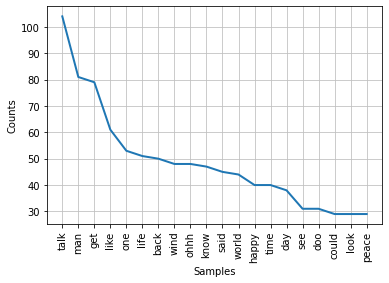
\includegraphics[width=\linewidth]{fd-all-KC.png}
		\caption{King Crimson, filtered}
		\label{fig:freq dist KC}
	\end{subfigure}%
	\begin{subfigure}{0.5\linewidth}
		\centering
		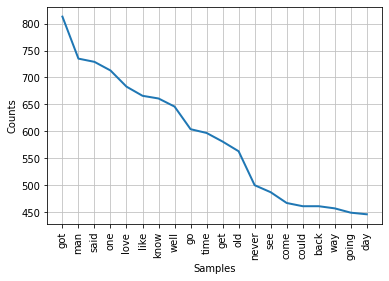
\includegraphics[width=\linewidth]{fd-all-JC.png}
		\caption{Johnny Cash, filtered}
		\label{fig:freq dist JC}
	\end{subfigure}
	
	\begin{subfigure}{0.5\linewidth}
		\centering
		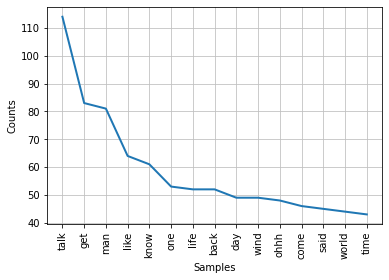
\includegraphics[width=\linewidth]{fd-all-KC-stem.png}
		\caption{King Crimson, filtered, stemmed}
		\label{fig:freq dist KC stem}
	\end{subfigure}%
	\begin{subfigure}{0.5\linewidth}
		\centering
		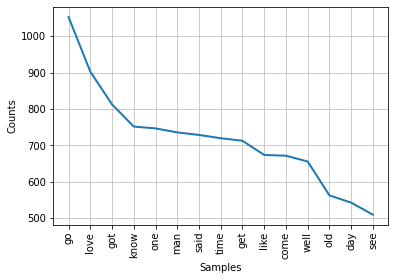
\includegraphics[width=\linewidth]{fd-all-JC-stem.png}
		\caption{Johnny Cash, filtered, stemmed}
		\label{fig:freq dist JC stem}
	\end{subfigure}
	\caption{Frequency distributions of words in artists' bodies of work with various methods of preprocessing applied.}
\end{figure*}